%!TEX root =  bgo-cam-ready.tex
% please do not delete or change the first line (needed by Csaba's editor)
%%%%%%%%%%%%%%%%%%%%%%%%%%%%%%%%%%%%%%%%%%%%%%%%%%%%%%%%%%%%%%%%%%%%%%%%%%%%%%% 
In this section we present the proof of \cref{thm:lb-convex}. 
Note that we will only prove lower bounds with the type-I oracle. According to \cref{thm:typered}, lower bounds for type-II can be directly attained by replacing $C_1$ of type-I with $C_1/\sqrt{d}$, given $[+1,-1]^d\subset \cK $.

\subsection{Proof of Theorem~\ref{thm:lb-convex} for the class of smooth convex functions $\F_{L,0}(\K)$}
\label{sec:appendix-lbconvex}
We will use a novel technique that will allow us to  reduce the $d$-dimensional case to the $1$-dimensional case (see later).
Thus, we start with the one-dimensional case.

\paragraph{Proof in one dimension:} 
We first prove the theorem for $\F = \F_{L,0}(\K) \cap\{ f:\R \to\R\,:\, \dom(f)=\cK\}$, where 
by the assumptions of the theorem, $L\ge 1/2$, $\K$ is convex and $[-1,1]\subset \K$, thereby proving a slightly
stronger result than stated.
For brevity, let $\Delta_n^{*}$ denote the minimax error $\Delta_n^*(\F, c_1,c_2)$. 
Throughout the proof, a $d$-dimensional normal distribution with mean $\mu$ and covariance matrix $\Sigma$ is denoted by $\normal(\mu, \Sigma)$.

We follow the standard proof technique of lower bounds: We define two functions $f_+, f_- \in \F$ with associated type-I gradient oracles $\gamma_+,\gamma_-$ such that the expected error of any deterministic algorithm can be bounded from below for the case when the environment is chosen uniformly at random from $\{(f_+,\gamma_+),(f_-,\gamma_-)\}$. By Yao's principle
\citep{Yao77:FOCS}, the same lower bound applies to the minimax error $\Delta_n^{*}$ even when randomized algorithms are also allowed.

The proof uses $(c_1,c_2)$ type-I oracles which have no memory.
In particular, we restrict the class of oracles to those that on input $(x,\delta)$ return 
a random gradient estimate 
\begin{equation}
\label{eq:oracle}
G(x,\delta) = \overline{\gamma}(x,\delta) + \xi
\end{equation}
with some map $\og: \cK \times [0,1)\to \R$,
where $\xi$ is a zero-mean normal random variable with variance $c_2(\delta):= C_2 \delta^{-q}$, satisfying the variance requirement, and drawn independently every time the oracle is queried.%
\footnote{The argument presented below is not hard to extend to the case when all observations are from a bounded set,
but this extension is left to the reader.}
The map $\og$, which will be chosen based on $f$ to satisfy the requirement on the bias.
The $Y$ value returned by the oracles is made equal to $x$.

Next we define the two target functions and their associated oracles. With a slight abuse of notation, we will use interchangeably the subscripts $+$ ($-$) and $+1$ ($-1$) for any quantities corresponding to these two environments, e.g., $f_+$ and $f_{+1}$ (respectively, $f_-$ and $f_{-1}$).
For $v \in \{\pm 1\}$, let
\begin{align}\label{eq:fvdef}
f_v(x) :=  \epsilon\left( x-v\right)+2\epsilon^2 \ln\left(1+e^{-\frac{x-v}{\epsilon}}  \right)\,,
%\text{ and } f_-(x) := \epsilon\left( x+1\right)+2\epsilon^2 \ln\left(1+e^{-\frac{x+1}{\epsilon}}  \right), 
\,\, x \in \cK\,.
\end{align}
%In what follows, we will slightly abuse notation by using $f_+$ ($f_-$) in place of $f_{+1}$ (resp., $f_{-1}$).
These functions, with the choice $\epsilon=0.1$, are shown in \cref{fig:lbfvdiff}. 
The idea underlying these functions is that they approximate $\epsilon|x-v|$, but with a prescribed smoothness.
The first and second derivatives of $f_v$ are
\begin{align*}
f'_v(x) &=\epsilon\, \dfrac{1-e^{-\frac{x-v}{\epsilon}}}{1+e^{-\frac{x-v}{\epsilon}}} \,, \qquad \text{ and } \qquad
f''_v(x) = \dfrac{2e^{-\frac{x-v}{\epsilon}} }{\left(  1+e^{-\frac{x-v}{\epsilon}}\right)^2}  \,
\end{align*}
(the functions were designed by choosing $f'_v$).
% we will slightly abuse notation by using $f_+$ ($f_-$) in place of $f_{+1}$ (resp., $f_{-1}$).
%%%%%%%%%%%%%%%%%%%%%%%%%%%%%%%%%%%%%%%%%%%%%%%%%%%%%%%%%%%%%%%%%%%%%%%%%%%%%%% 
From the above calculation, it is easy to see that $0 \le f''(x) \le 1/2$; thus $f_v$ is $\frac{1}{2}$-smooth, and so $f_v\in \F$.

For $f_v, v\in\{-1,+1\}$, the gradient oracle we consider is defined as $\gamma_v(x,\delta)=\og_v(x,\delta)+\xi_\delta$ with $\xi_\delta \sim \normal(0,\frac{C_2}{\delta^q})$ selected independently for every query, where $\og_v$ is a biased estimate of the gradient $f'_v$. 
The derivatives of $f_+$ and $f_-$ are shown in \cref{fig:lbfvdiff}; we define the ''bias'' in $\og_v$ to move the gradients closer to each other:
The idea is to shift $f_+'$ and $f_-'$ towards each other, with the shift depending on the allowed bias $c_1(\delta) = C_1\delta^p$.
In particular, since $f_+'\le f_-'$, $f_+'$ is shifted up, while $f_-'$ is shifted down. 
However, the shifted up version of $f_+'$ is clipped for positive $x$ so that it never goes above the 
shifted down version of $f_-'$, cf. \cref{fig:fprime}.
 By moving the curves towards each other, algorithms which rely on the obtained oracles
will have an increasingly harder time (depending on the size of the shift) to distinguish whether the function optimized is $f_+$ or $f_-$. Since
\begin{align*}
0\le f_-'(x) - f_+'(x) \le \sup_{x} f_-'(x) - \inf_x f_+'(x) = 2\epsilon\,,
\end{align*}
we don't allow shifts larger than $\epsilon$ (so no crossing over happens), leading to the following formal definitions:


%making it challenging for any algorithm to distinguish $f_+$ and $f_-$ based on observations from $\gamma_+$ or $\gamma_-$, respectively:
\begin{align}
\overline{\gamma}_+(x,\delta) = 
	\begin{cases}
	f_+'(x) + \min(\epsilon,C_1\delta^p)\,, & \text{if } x<0\,; \\
	\min\big\{f_+'(x) + \min(\epsilon,C_1\delta^p), f_-'(x) - \min(\epsilon,C_1\delta^p)\big\}\,, & \text{otherwise}\,,
	\end{cases}
	\label{eq:og1}
\end{align}
and
\begin{align}
\overline{\gamma}_-(x,\delta) = 
	\begin{cases}
	f_-'(x) - \min(\epsilon,C_1\delta^p)\,, & \text{if } x>0\,; \\
	\max\big\{f_-'(x) - \min(\epsilon,C_1\delta^p), f_+'(x) + \min(\epsilon,C_1\delta^p)\big\}\,, & \text{otherwise}\,.
	\end{cases}
	\label{eq:og2}
\end{align}
We claim that the oracle $\gamma_v$ based on these functions
 is indeed a $(c_1,c_2)$ type-I oracle, with $c_1(\delta)=C_1\delta^p$ and $c_2(\delta)=\frac{C_2}{\delta^q}$. The variance condition is trivial.
To see that $c_1(\delta) = C_1\delta^p$ works, 
notice that $\gamma_v(x,\delta) = -\gamma_{-v}(-x,\delta)$ and $f_v'(x) = -f_{-v}'(-x)$. Thus,
$|\overline{\gamma}_+(x,\delta)-f_+'(x)| = |\overline{\gamma}_-(-x,\delta)-f_-'(-x)|$, hence it suffices to consider $v=+1$.
The bias condition trivially holds for $x<0$. For $x\ge 0$, using that $f'_+(x) \le f'_-(x)$, we get
$f'_+(x) - \min(\epsilon,C_1\delta^p) \le \og_+(x,\delta) \le f'_+(x) + \min(\epsilon,C_1\delta^p)$, showing 
$|\overline{\gamma}_+(x,\delta)-f_+'(x)|  \le C_1 \delta^p$.
Thus, $\gamma_v$ is indeed an oracle with the required properties.


 \begin{figure}
   \centering
	\begin{tabular}{cc}
	  \begin{subfigure}[b]{0.5\textwidth}
 \centering
   \scalebox{0.8}{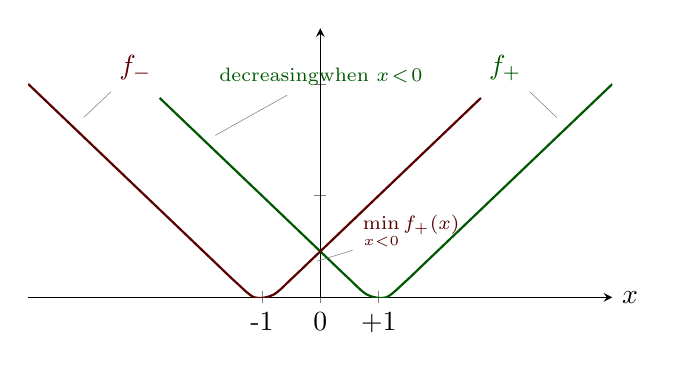
\begin{tikzpicture}
   \begin{axis}[width=9cm,height=5cm,
          %  grid = major,         
            axis y line=middle,
            axis x line=bottom,
						xlabel={$x$},
						every axis x label/.style={at={(current axis.right of origin)},anchor=west},
						%x label style={at={(4,-0.1)}},
						%ylabel={$f_v$},
           % grid style={dashed, gray!30},
            %xmin=-3,     % start the diagram at this x-coordinate
            %xmax=3,    % end   the diagram at this x-coordinate
						ymax=0.5,
						xtick={-1,0,1},
            xticklabels={-1,0,+1},
            yticklabels=\empty
            ]
           \addplot[domain=-2.75:5, green!35!black, thick,smooth] 
              {0.1*(x-1) + 2*0.01*ln(1+exp(-10*(x-1)))} node [pos=0.9,pin={135:$f_+$}] {} node [pos=0.1,pin={85:{\makecell{\scriptsize decreasing\\\scriptsize when $x\!<\!0$}}}] {}; 
            \addplot[domain=-5:2.75, red!35!black,thick,smooth] 
              {0.1*(x+1) + 2*0.01*ln(1+exp(-10*(x+1)))} node [pos=0.1,pin={45:$f_-$}] {} node [pos=0.615,pin={5:\makecell{\scriptsize$\min\limits_{x<0} f_+(x)$}}] {}; 
   \end{axis}
   \end{tikzpicture}}
	\caption{Plot of $f_+$ and $f_-$ with $\epsilon=0.1$}
\label{fig:lbfvdiff}
	  \end{subfigure}
	&
	  \begin{subfigure}[b]{0.5\textwidth}
 \centering
   \scalebox{0.8}{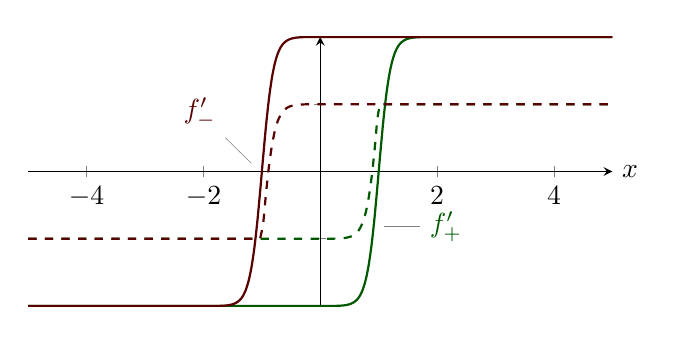
\begin{tikzpicture}
   \begin{axis}[width=9cm,height=5cm,
          %  grid = major,         
            axis y line=middle,
            axis x line=middle,
						xlabel={$x$},
						every axis x label/.style={at={(current axis.right of origin)},anchor=west},
						%x label style={at={(4,-0.1)}},
						%ylabel={$f_v$},
           % grid style={dashed, gray!30},
            %xmin=-3,     % start the diagram at this x-coordinate
            %xmax=3,    % end   the diagram at this x-coordinate
						%xtick={-1,0,1},
            %xticklabels={-1,0,+1},
            yticklabels=\empty,
            samples=200
            ]
           \addplot[domain=-5:5, green!35!black, thick,smooth] 
              {0.1*(1-exp(-10*(x-1)))/(1+exp(-10*(x-1)))} node [pos=0.59,pin={0:$f'_+$}] {}; 
            \addplot[domain=-5:5, green!35!black, thick,dashed, smooth] 
              {
              (x<0)*
               (0.1*(1-exp(-10*(x-1)))/(1+exp(-10*(x-1)))+0.05)
               +
               (x>=0)*min(
	               0.1*(1-exp(-10*(x+1)))/(1+exp(-10*(x+1)))-0.05,
    		           0.1*(1-exp(-10*(x-1)))/(1+exp(-10*(x-1)))+0.05
               ) 
              } ;  % dashed green 
            \addplot[domain=-5:5, red!35!black,thick,smooth] 
              {0.1*(1-exp(-10*(x+1)))/(1+exp(-10*(x+1)))} node [pos=0.4,pin={135:$f'_-$}] {}; 
              \addplot[domain=-5:5, red!35!black,thick,dashed] 
              {
              (x>0)*
              (0.1*(1-exp(-10*(x+1)))/(1+exp(-10*(x+1)))-0.05)
              +
              (x<=0)*max(
	               0.1*(1-exp(-10*(x+1)))/(1+exp(-10*(x+1)))-0.05,
    		           0.1*(1-exp(-10*(x-1)))/(1+exp(-10*(x-1)))+0.05
              )
              };
							%\node at (axis cs:1,0.5) {P3};
   \end{axis}
   \end{tikzpicture}}
	\caption{Plot of $f'_+$ and $f'_-$ with $\epsilon=0.1$. 
	The dashed lines show
	$\overline{\gamma}_v(\cdot,\delta)$ for $C_1\delta^p=\epsilon$, 
	$v\in \{\pm 1\}$.}
	\label{fig:fprime}
\end{subfigure}
	\end{tabular}
\end{figure}

To bound the performance of any algorithm in minimizing $f_v, v \in \{\pm 1\}$, notice that $f_v$ is minimized at $x^*_v = v$, with $f_v(v) = 2 \epsilon^2 \ln 2$.
Next we show that if $x$ has the opposite sign of $v$, the difference $f_v(x)-f_v(x_v^*)$ is ``large''.
This will mean that if the algorithm cannot distinguish between $v=+1$ and $v=-1$, it necessarily chooses a
highly suboptimal point for either of these cases.

Since $v f_v$ is decreasing on $\{x\,:\, xv \le 0\}$, we have
\begin{align*}
M_v :=&\,\, \min_{x:xv \le 0} f_v(x) - f_v(v) 
=   f_v(0) - f_v(v)  
=  \epsilon\left(-v + 2\epsilon\ln\dfrac{1+e^{\frac{v}{\epsilon}}}{2}\right). \nonumber %\label{eq:lbfvdiff2}
\end{align*}
%Above, the equality in \eqref{eq:lbfvdiff} can be inferred as follows: Suppose $v=+1$. As illustrated in Figure \ref{fig:lbfvdiff}, $\min_{x:xv<0} f_v(x)$ is achieved at $x=0$ due to monotonicity of $f_v$. A similar argument works for $v=-1$ as well. 
%This can also be seen from the plot of $f_+$ to the left of $+1$ and of $f_-$ to the right of $-1$ in Figure \ref{fig:lbfvdiff}. 
Let $h(v) = -v + 2\epsilon\ln\dfrac{1+e^{\frac{v}{\epsilon}}}{2}$.
Simple algebra shows that $h$ is an even function, that is, $h(v) = h(-v)$. Indeed,
\begin{align*}
h(v) = -v + 2\,\epsilon\,\ln\left(e^{\frac{v}{\epsilon}} \dfrac{1+e^{-\frac{v}{\epsilon}}}{2}\right)
= -v + 2\,\epsilon\, \dfrac{v}{\epsilon}  + 2\,\epsilon\,\ln\dfrac{1+e^{-\frac{v}{\epsilon}}}{2}
=  h(-v)\,.
\end{align*}
Specifically, $h(1) = h(-1)$ and thus
\begin{align*}
M_+= M_- = \epsilon\left(-1 + 2\epsilon\ln\dfrac{1+e^{\frac{1}{\epsilon}}}{2}\right)\,.
\end{align*}
From the foregoing, when $xv \le 0$ and $\epsilon<\dfrac{1}{4\ln 2}$,  we have
\begin{align*}
f_v(x)-f_v(x_v^*) \ge \epsilon\left( -1 +2\epsilon \ln\dfrac{1+e^{\frac{1}{\epsilon}}}{2}  \right)> \dfrac{\epsilon}{2}.
\end{align*}
Hence,
%Using the fact that $f_+$ and $f_-$ are strongly convex with associated constant $\left(\dfrac{\epsilon}{2}\right)$, we obtain
\begin{align}
  f_v(x) - f_v(x^*_v)
  \ge \dfrac{\epsilon}{2}  \indic{x v  < 0}. \label{eq:fv-lb}
\end{align}
% Similarly,   $f_-(x) - f_-(x^*_-) \ge  \dfrac{\epsilon}{2}  \indic{x  >0}$.


Given the above definitions and \eqref{eq:fv-lb}, by Yao's principle, the minimax error \eqref{eq:minimaxerrdef} is lower bounded by
%\footnote{$f_{+1} \equiv f_+$ and $f_{-1}\equiv f_-$.}:
\begin{align}
\MoveEqLeft 
\Delta_n^{*} %\nonumber\\
  \ge  \inf_{\A} \,  \E[f_V(\hat X_n) - \inf_{x \in X}  f_V(x)]
  \ge \inf_{\A} \, \dfrac{\epsilon}{2}\,  \P(\hat X_n V < 0)\,,
  \label{eq:avg-bd}
  \end{align}
where $V \in \{\pm 1\}$ is a random variable, $\hat{X}_n$ is the estimate of the algorithm after $n$ queries to the oracle $\gamma_V$ for $f_V$, the infimum is taken over all deterministic algorithms, and the expectation is taken with respect to the randomness in $V$ and the oracle. More precisely, the distribution above is defined as follows:

Consider a fixed $(c_1,c_2)$ type-I oracle $\gamma$ satisfying \eqref{eq:oracle} and a deterministic algorithm $\A$. Let $x_t^{\A}$ (respectively, $\delta_t^{\A}$) denote the map from the algorithm's past observations that picks the point (respectively, accuracy parameter $\delta$), which are sent to the oracle in round $t$. Define the probability space $(\Omega, \B, P_{\A,\gamma})$ with
$\Omega = \R^n\times \{-1,1\}$,  its associated Borel sigma algebra $\B$, where the probability measure
$P_{\A,\gamma}$ takes the form $P_{\A,\gamma} := p_{\A,\gamma} d(\lambda \times m)$, 
where
	$\lambda$ is the Lebesgue measure on $\R^n$, 
	$m$ is the counting measure on $\{\pm 1\}$ and 
	$p_{\A,\gamma}$ is the density function defined by
\begin{align*}
p_{\A,\gamma}(g_{1:n}, v) 
&= \frac{1}{2} \bigg( p_{\A,\gamma}(g_n \mid g_{1:n-1})
		\cdot \ldots \cdot p_{\A,\gamma }(g_{n-1} \mid g_{1:n-2}) \cdot \ldots \cdot p_{\A,\gamma}(g_1) \bigg) \\
&=  \frac{1}{2} \bigg( p_{\N}\big(g_n - 
				\overline{\gamma}(x_n^{\A}(g_{1:n-1}),\delta_n^{\A}(g_{1:n-1})),c_2(\delta_n^{\A}(g_{1:n-1}))\big) \cdot
%  &\times p_{\normal(0,\sigma^2)}(g_{n-1} - \gamma(\A_n(g_{1:n-2}))) \times \ldots \\
									 \ldots \cdot  p_{\N}\big(g_1 - \overline{\gamma}(x_1^{\A},\delta_1^{\A}),c_2(\delta_1^{\A})\big) \bigg),
\end{align*}
where $v\in\{-1,1\}$ and $p_{\N}(\cdot,\sigma^2)$ is the density function of a $\normal(0,\sigma^2)$ random variable.
Then the expectation in \eqref{eq:avg-bd} is defined w.r.t. the distribution $\P:= \dfrac{1}{2} \left(P_{\A, \gamma_+} \indic{v=+1} + P_{\A, \gamma_-}\indic{v=-1}\right)$ and $V: \Omega \to \{\pm 1 \}$ is defined by $V(g_{1:n},v) = v$.%
\footnote{Here, we are slightly abusing the notation as $\P$ depends on $\A$, but the dependence is suppressed.
In what follows, we will define several other distributions derived from $\P$, which will all depend on $\A$, but
for brevity this dependence will also be suppressed.
The point where the dependence on $\A$ is eliminated will be called to the reader's attention.}
Define $\P_{+}(\cdot) := \P(\cdot\mid V=1)$, $\P_{-}(\cdot) := \P(\cdot\mid
V=-1)$. 
% \todoa{This notation is somewhat confusing given the previous conventions.}
% \todoc{Better? I moved the definition upfront. I don't think there is much to complain about this definition. It is pretty clear.
% If you want, change it, but then do it consistently (and be . I have no time to change this and I have no idea what is that you would like.}
From \eqref{eq:avg-bd}, we obtain
\begin{align}
\Delta_n^{*}  
%\ge & \inf_{\A} \dfrac{\epsilon}{4}\,  \P(\hat X_n V < 0), \label{eq:strong-convex-bd}\\
  \ge & \inf_{\A} \dfrac{\epsilon }{4} \, \left(\P_{+}(\hat X_n < 0) + \P_{-}(\hat X_n > 0)\right), \label{eq:Pplus}\\
  \ge &\inf_{\A} \dfrac{\epsilon }{4} \,\left(1 - \tvnorm{\P_{+}- \P_{-}}\right), \label{eq:lecam}\\
  \ge &\inf_{\A} \dfrac{\epsilon }{4}  \,\left( 1 - \left(\frac12\dkl{P_{+}}{P_{-}}\right)^{\frac{1}{2}}\right), \label{eq:pinsker}
\end{align}
where 
 \eqref{eq:Pplus} uses the definitions of $\P_+$ and $\P_-$, $\tvnorm{\cdot}$ denotes the total variation distance,  
 \eqref{eq:lecam} follows from its definition, while \eqref{eq:pinsker} follows from Pinsker's inequality. 
It remains to upper bound $\dkl{P_{+}}{P_{-}}$.


%%%%%%%%%%%%%%%%%%%%%%%%%%%%%%%%%%%%%%%%%%%%%%%%%%%%%%%%%%%%%%%%%%%%%%%%%%%%%%% 
Define $G_t$ to be the $t$th observation of $\A$. Thus, $G_t:\Omega \to \R$, with $G_t( g_{1:n}, v) = g_t$.
Let $P_+^t(g_1,\dots,g_t)$ denote the joint distribution of $G_1,\dots,G_t$ conditioned on $V=+1$.
Let $P_{+}^t(\cdot\mid g_1,\ldots,g_{t-1})$ denote the distribution of $G_t$ conditional on $V=+1$ and $G_1=g_1,\ldots,G_{t-1}=g_{t-1}$. Define  $P_{-j}^t(\cdot\mid g_1,\ldots,g_{t-1})$ in a similar fashion.
Then, by the chain rule for KL-divergences, we have
\begin{align}
\label{eq:dklchain}
&\dkl{P_{+}}{P_{-}}= \sum_{t=1}^n \int_{\R^{t-1}} \dkl{P_{+}^t(\cdot\mid g_{1:t-1})}{P_{-}^t(\cdot\mid g_{1:t-1})} d P_{+}^t( g_{1:t-1}).
\end{align}
By the oracle's definition on $V=+1$ we have
$G_t \sim  \normal(\overline{\gamma}_{+}(x^{\cA}_t(G_{1:t-1}),\delta_t^{\A}(G_{1:t-1})),c_2(\delta^{\A}_t(G_{1:t-1})))$, i.e., 
$P_{+}^t(\cdot\mid g_{1:t-1})$ is the normal distribution with mean 
$\overline{\gamma}_{+}(x^{\cA}_t(G_{1:t-1}),\delta^{\A}_t(G_{1:t-1}))$ and variance $c_2(\delta^{\A}_t(G_{1:t-1}))$.
%, where $A(g_{1:t-1})$ denotes the point chosen by the algorithm given observations $g_1,\ldots, g_{t-1}$ and $\gamma_{+}$ is the gradient oracle defined earlier. 
Using the shorthands $x_t^{\A}:=x^{\A}_t(g_{1:t-1})$, $\delta_t^{\A}:=\delta^{\A}_t(g_{1:t-1})$,
we have
\begin{align*}
\dkl{P_{+}^t(\cdot\mid g_{1:t-1})}{P_{-}^t(\cdot\mid g_{1:t-1})}
& =\dfrac{(\overline{\gamma}_{+}(x_t^{\A},\delta_t^{\A}) - \overline{\gamma}_{-}(x_t^{\A},\delta_t^{\A}))^2}{2 c_2(\delta^{\A}_t)}\,,
\end{align*}
as the KL-divergence between normal distributions $\normal(\mu_1,\sigma^2)$ and $\normal(\mu_2,\sigma^2)$ is equal to $\dfrac{(\mu_1 - \mu_2)^2}{2 \sigma^2}$.

It remains to upper bound the numerator. For $(x,\delta)\in \R\times (0,1]$, first note that $\gamma_+(x,\delta)\le \gamma_-(x,\delta)$. Hence,
\begin{align*}
|\gamma_+(x,\delta)-\gamma_-(x,\delta)|
& =  \gamma_-(x,\delta) - \gamma_+(x,\delta) \\
& < \sup_x \gamma_-(x,\delta) - \inf_x \gamma_+(x,\delta) \\
& = \lim_{x\to\infty} \gamma_-(x,\delta) - \lim_{x\to-\infty} \gamma_+(x,\delta) \\
& = \epsilon - \epsilon\wedge C_1\delta^p - (-\epsilon + \epsilon \wedge C_1\delta^p)\\
& = 2\epsilon - 2\epsilon \wedge C_1\delta^p\\
& \le 2(\epsilon - C_1\delta^p)^+\,, \numberthis \label{eq:gdiff-ub}
\end{align*}
where $(u)^+ = \max(u,0)$ is the positive part of $u$.
%\todoc{I believe you don't want $(u)_+$, which is the standard notation, because it collides with or use of $+$ and $-$ as an index.  Is this really such a big issue? I have a slight preference for $(u)_+$. But fine. If you are determined, just take out this note.}

%where $\delta(g_{1:t-1})$ is the tolerance parameter chosen by $\A$, based on the observations $g_{1:t-1}$. 
From the above, using the abbreviations $x_t^{\A} = x^{\A}_t(g_{1:t-1})$ and $\delta_t^{\A} = \delta^{\A}_t(g_{1:t-1})$ (effectively fixing $g_{1:t-1}$ for this step),
\begin{align}
\dkl{P_{+}^t(\cdot\mid g_{1:t-1})}{P_{-}^t(\cdot\mid g_{1:t-1})}
%& =\dfrac{(\overline{\gamma}_{+}(x_t^{\A},\delta_t^{\A}) - \overline{\gamma}_{-}(x_t^{\A},\delta_t^{\A}))^2}{2 c_2(\delta^{\A}_t)}
%				\label{eq:dkgauss1}\\
& < \dfrac{2\{(\epsilon-C_1(\delta^{\A}_t)^p)^+\}^2\,(\delta^{\A}_t)^q}{C_2}\label{eq:dkgauss}\\
& \le  \sup_{\delta>0} \dfrac{2\{(\epsilon-C_1\delta^p)^+\}^2\,\delta^q}{C_2} \label{eq:supdelta}\,,
\end{align}
where inequality \eqref{eq:dkgauss} follows from \eqref{eq:gdiff-ub}. Notice that the right-hand side of the above inequality does not depend on the algorithm anymore.

Now, observe that 
$\sup_{\delta> 0} \{(\epsilon - C_1 \delta^p)^+\}^2 \delta^q = \sup_{(\epsilon/C_1)^{1/p} \ge \delta> 0} (\epsilon - C_1 \delta^p)^2 \delta^q$. From this we obtain
\begin{align}
\delta_*=\left(\frac{\epsilon q}{C_1(2p+q)}\right)^{1/p}. \label{eq:deltastar}
\end{align}
%\todoc[inline]{
%Here is the calculation to get this:
%I defined $u = \delta^q$, writing $(\epsilon-C_1 \delta^p)^2 \delta^q = (\epsilon-C_1 u^z)^2 u 
%= \epsilon^2 u- 2C_1 \epsilon u^{z+1} + C_1^2 u^{2z+1}
%= :f(u)$.
%The first order optimality criterion is
%$0 = f'(u) = C_1^2(2z+1) (u^z)^2 - 2 C_1 (z+1) \epsilon u^z + \epsilon^2$, from which I get
%$(u^z)_{1,2} = \frac{2C_1(z+1)\epsilon \pm 2 C_1 z \epsilon}{2C_1^2(2z+1)}$,
%that is $u^z_1 = \frac{\epsilon }{C_1 (2z+1)}$, $u^z_2 = \frac{\epsilon}{C_1}$.
%Note that at the end-points of the interval $[0,(\epsilon/C_1)^{1/z}]$
%the function $f$ equals zero, while inside the interval it takes on positive values.
%We see that the larger endpoint of this interval is $u_2$. Hence, the function must have a 
%unique maximum in this interval at $u_1$. 
%Thus,  $\delta_* = u_1^{1/q}$, i.e., $\delta_* = ( \frac{\epsilon }{C_1 (2z+1)})^{1/p}$.
%The condition $\delta_*\le (\epsilon/C_1)^{1/p}$ gives $2z+1\ge 1$, which holds no matter the values of $p,q$.
%Therefore, 
% $\{(\epsilon-C_1 \delta_*^p)^+\}^2 \delta_*^q = (\epsilon-C_1 \delta_*^p)^2 \delta_*^q$.
%}
%Here the condition $\delta_* \le 1$ is satisfied if $ \epsilon \le C_1$, which will hold by our choice of $\epsilon$.
Note that $C_1\delta_*^p\le \epsilon$, hence
$\max_{\delta> 0} \{(\epsilon - C_1 \delta^p)^+\}^2 \delta^q =  (\epsilon-C_1 \delta_*^p)^2 \delta_*^q$.
Plugging \eqref{eq:supdelta} into \eqref{eq:dklchain} and using this last observation we obtain
\begin{align}
\dkl{P_{+}}{P_{-}} \le \dfrac{2n}{C_2} \,(\epsilon-C_1\delta_*^p)^2\, \delta_*^q\,.
\end{align}
Note that the above bound holds uniformly over all algorithms $\A$. 
Substituting the above bound into \eqref{eq:pinsker}, we obtain 
\begin{align}
\Delta_n^{*}
  \ge  \dfrac{\epsilon}{4} \left(1 - \sqrt{
    n}  \dfrac{ (\epsilon-C_1\delta_*^p)\delta_*^{q/2}}{\sqrt{C_2}}
  \right)
  = \frac{\epsilon}{4}\left(1-\sqrt{n} K_1 \epsilon^{\frac{2p+q}{2p}}\right)\,,\label{eq:final-lower-bd}
\end{align}
where $K_1= \frac{2p}{\sqrt{C_2}(2p+q)}\left(\frac{q}{C_1(2p+q)}\right)^{\frac{q}{2p}}$.
%where we used again that $C_1 \delta_*^p\le \epsilon$.
%%%%%%%%%%%%%%%%%%%%%%%%%%%%%%%%%%%%%%%%%%%%%%%%%%%%%%%%%%%%%%%%%%%%%%%%%%%%%%%
% \paragraph{Derivations of rates:}
%  Optimizing over $\epsilon$ in \eqref{eq:final-lower-bd}, we get
% $ \left(\dfrac{\delta^{-q/2}C_2}{4\sqrt{n}} + \dfrac{C_1\delta^p}{2}\right)$. We choose
% \[
% \epsilon^* = \left(\dfrac{\delta^{-q/2}C_2}{4\sqrt{n}} + C_1\delta^p\right)
% \]
% to guarantee that $\epsilon^*>C_1 \delta^p$.
% 
%  Plugging in $\epsilon^*$, we obtain
%  \[
%  \Delta_n^{*}
%  \ge \frac18 \left(\dfrac{\delta^{-q/2}C_2}{2\sqrt{n}} + C_1\delta^p \right).
%  \]
% 
% Substituting $p=1$ and $q=2$, we obtain
% \[
% \delta^*= \sqrt{\dfrac{C_2}{2C_1}}\dfrac{1}{n^{\frac{1}{4}}} \text{ and } 
% \Delta_n^{*} \ge \left(\dfrac{\sqrt{2C_1C_2}}{4}\right)\dfrac{1}{n^{\frac{1}{4}}}.
% \]
% 
% On the other hand, substituting $p=q=2$, we obtain
% \[
% \delta^*= \left(\dfrac{C_2}{2C_1}\right)^{\frac{1}{3}}\dfrac{1}{n^{\frac{1}{6}}} \text{ and } \Delta_n^{*} \ge \left(\dfrac{C_1^{\frac{1}{3}}C_2^{\frac{2}{3}}}{4\, 2^{\frac{1}{3}}}\right)\dfrac{1}{n^{\frac{1}{3}}}.
% \]

%\paragraph{Derivation of the rates uniformly for all $\delta$:}
%From the above, given $\epsilon \le C_1$, we have the following lower bound on the minimax error $\Delta_n^{*}$:
 
By choosing $\epsilon = \left(\frac{2p}{\sqrt{n} K_1(4p+q)} \right)^{\frac{2p}{2p+q}}$, we see that 
\begin{align}
\Delta_n^* \ge \frac{2p+q}{4(4p+q)}\left(\frac{2p}{\sqrt{n} K_1(4p+q)} \right)^{\frac{2p}{2p+q}} = \frac{\left(2p+q\right)^2}{4q^{\frac{q}{2p+q}}\left(4p+q\right)^{\frac{4p+q}{2p+q}}}C_1^{\frac{q}{2p+q}} C_2^{\frac{p}{2p+q}}  n^{-\tfrac{p}{2p+q}} \,.
\label{eq:lb-pq}
\end{align}
%as long as $n \ge \frac{C_2 (2z+1)^{2+1/z}}{C_1^2 (4z+1)^2}$.
%The conditions on $n$ for the above bound to hold are:
%\begin{align}
%\frac{1}{\sqrt{d}}\left(\frac{1}{\sqrt{n} K_1} \right)^{\frac{p}{p+\frac{q}{2}}}\le \min\left( \frac{C_1 (2p+q)}{q}, \frac{2z+1}{C_1^{2z-1}(z+1)^z}\right).
%\end{align}
%The above conditions on $n$ can be inferred from (i) the requirement on  $\epsilon$ in \eqref{eq:deltastar}, (ii) assumption $\delta \le 1$ in Definition \ref{def:oracle1},  and (iii) the optimal choice of $\epsilon$ above.

Now, when $p=1$ and $q=2$, the lower bound in \eqref{eq:lb-pq} simplifies to 
\[
\Delta_n^{*} \ge \dfrac{ 1}{3\sqrt{3}} C_1^{1/2}C_2^{1/4} n^{-1/4} \,.
\]
On the other hand, for $p=q=2$, we obtain 
\[
\Delta_n^{*} \ge  \frac{9}{20}\left(\frac{1}{25}\right)^{1/3}C_1^{1/3}C_2^{1/3} n^{-1/3}\,.
\]

%%%%%%%%%%%%%%%%%%%%%%%%%%%%%%%%%%%%%%%%%%%%%%%%%%%%%%%%%%%%%%%%%%%%%%%%%%%%%%%
%%%%%%%%%%%%%%%%%%%%%%%%%%%%%%%%%%%%%%%%%%%%%%%%%%%%%%%%%%%%%%%%%%%%%%%%%%%%%%%
%%%%%%%%%%%%%%%%%%%%%%%%%%%%%%%%%%%%%%%%%%%%%%%%%%%%%%%%%%%%%%%%%%%%%%%%%%%%%%%
\paragraph{Generalization to $d$ dimensions:}
To prove the $d$-dimensional result, we introduce a new device which allows us to relate the minimax error of the $d$-dimensional problem to that of the $1$-dimensional problem.
The main idea is to use separable $d$-dimensional functions and oracles and show that if there exists an algorithm with a small loss for a rich set of separable functions and oracles, then there exists good one-dimensional algorithms for the one-dimensional components of the functions and oracles.

This device works as follows: First we define one-dimensional functions.
For $1\le i \le d$, let $\cK_i \subset \R$ be nonempty sets, 
and for each $v_i \in V := \{\pm 1\}$, let $f_v^{(i)}: \cK_i \to \R$.
%(later we will use $V_i=\{\pm 1\}$ and $f_v^{(i)}$ will be the functions constructed for the $1$-dimensional case with $\{-1,+1\}\subset \cK_i\subset \R$). Further, let $\gamma_{v_i}^{(i)}$ be a gradient oracle that the algorithms can use when 
%the function to be optimized is $f_v^{(i)}$. 
%
Let $\cK = \times_{i=1}^d \cK_i$ and for $v = (v_1,\dots,v_d) \in V^d$, let $f_v: \cK \to \R$ be defined by
\begin{align}
f_v(x) = \sum_{i=1}^d f^{(i)}_{v_i}(x_i), \qquad x\in \cK\,. \label{eq:sepfdef}
\end{align}
Without the loss of generality, we assume that $\inf_{x_i \in \cK_i} f_{v_i}^{(i)}(x_i) = 0$, and hence $\inf_{x\in \times_{i=1}^d \cK_i} f_{v}(x) = 0$, so that the optimization error of the algorithm producing $\hat{X}_n \in\cK$  as the output is $f_v^{(i)}(\hat{X}_{n,i})$ and $f_v(\hat{X}_{n})$, respectively.
We also define a $d$-dimensional \emph{separable} oracle $\gamma_v$  as follows: 
The oracle  is obtained from ``composing'' the $d$ one-dimensional oracles, $(\gamma_{v_i}^{(i)})_{i}$.
In particular, the $i$th component of the response of $\gamma_v$ 
given the history of queries $(x_{t},\delta_{t},\dots,x_1,\delta_1)\in (\cK \times [0,1))^t$
is defined as the response of $\gamma^{(i)}_{v_i}$ 
given the history of queries $(x_{t,i},\delta_{t},\dots,x_{1,i},\delta_1)\in (\cK_i\times [0,1))^t$.
This definition is so far unclear about the randomization of the oracles. 
In fact, it turns out that the one-dimensional oracles can even use the same randomization (i.e.,
their output can depend on the same single uniformly distributed random variable $U$), but they could also use separate randomization: our argument will not depend on this.
\newcommand{\sep}{\mathrm{sep}}
Let $\Gamma^{(i)}(f_{v_i}^{(i)},c_1,c_2)$ 
denote a non-empty set of $(c_1,c_2)$ type-I oracles for objective function $f^{(i)}_{v_i}:\cK_i \to \R$,
and let us denote by $\Gamma_\sep(f_v,c_1,c_2)$ the set of separable oracles for the function $f_v$ 
defined above.
We also define $\cF_\sep = \{ f\,: \, f(x) = \sum_{i=1}^d f^{(i)}_{v_i}(x_i), x\in \cK, v_i\in V_i \}$, the set of componentwise separable functions.
Note that when $\norm{\cdot} = \norm{\cdot}_2$ is used in the definition of type-I oracles then
$\Gamma_\sep(f_v,c_1/\sqrt{d},c_2/d) \subset \Gamma(f_v,c_1,c_2)$.

Let an algorithm $\A$ interact with an oracle $\gamma$.
We will denote the distribution of the output $\hat{X}_n$ of $\A$
at the end of $n$ rounds by $F_{\A,\gamma}$ 
(we fix $n$, hence the dependence of $F$ on $n$ is omitted).
Thus, the expected optimization error of $\A$ on a function $f$ with zero optimal value is 
\begin{align*}
L^{\A}(f,\gamma) = \int f(x) F_{\A,\gamma}(d x)\,.
\end{align*}
Note that this definition applies both in the one and the $d$-dimensional cases.
For $v\in V^d$, we introduce the abbreviation
\begin{align*}
L^{\A}(v) = L^{\A}(f_v,\gamma_v)\,.
\end{align*}
We also define
\newcommand{\tL}{\tilde{L}}
\begin{align*}
\tL^{\A}_i(v) = \int f_{v_i}^{(i)}( x_i ) F_{\A,\gamma_v}(d x)\,
\end{align*}
so that 
\begin{align*}
L^{\A}(v) = \sum_{i=1}^d \tL^{\A}_i(v)\,.
\end{align*}
Also, for $v_i \in V$ and a one-dimensional algorithm $\A$, we let
\begin{align*}
L^{\A}_i(v_i) = L^{\A}(f_{v_i}^{(i)}, \gamma_{v_i}^{(i)})\,.
\end{align*}
Note that while the domain of $\tL^{A}_i$ is $V^d$, the domain of $L^{\A}_i$ is $V$,
while both express an expected error measured against $f_{v_i}^{(i)}$.
In fact,  $\tL^{A}_i$ depends on $v$ because the algorithm $\A$ uses the $d$-dimensional oracle $\gamma_v$, which depends on $v$ (and not only on $v_i$) and thus algorithm $\A$ could use information returned by $\gamma_{v_j}^{(j)}$, $j\ne i$. In a way our proof shows that using this information cannot help a $d$-dimensional algorithm on a separable problem, a claim that we find rather intuitive, and which we now formally state and prove.

\begin{lemma}[``Cross-talk'' does not help in separable problems]
\label{lemma:sep}
Let %$V= \times_{i=1}^d V_i$, 
$(f_v)_{v\in V^d}, f_v \in \cF_\sep$, $(\gamma_v)_{v\in V^d}, \gamma_v \in \Gamma_\sep(f_v,c_1,c_2)$ be separable for some arbitrary functions $c_1,c_2$, and let $\A$ be any $d$-dimensional algorithm. Then there exist  $d$ one-dimensional algorithms, $\A_i^*$, $1\le i \le d$ (using only one-dimensional oracles),
such that 
\begin{align}
\label{eq:onedimlb}
% \begin{split}
% \MoveEqLeft 
&\max_{v\in V} L^{\A}(v) 
\ge   \max_{v_1\in V_1} L_1^{\A_1^*}(v_1) + \dots + \max_{v_d\in V_d} L_d^{\A^*_d}(v_d)\,.
% \end{split}
\end{align}
\end{lemma}
\begin{figure}
\begin{center}
	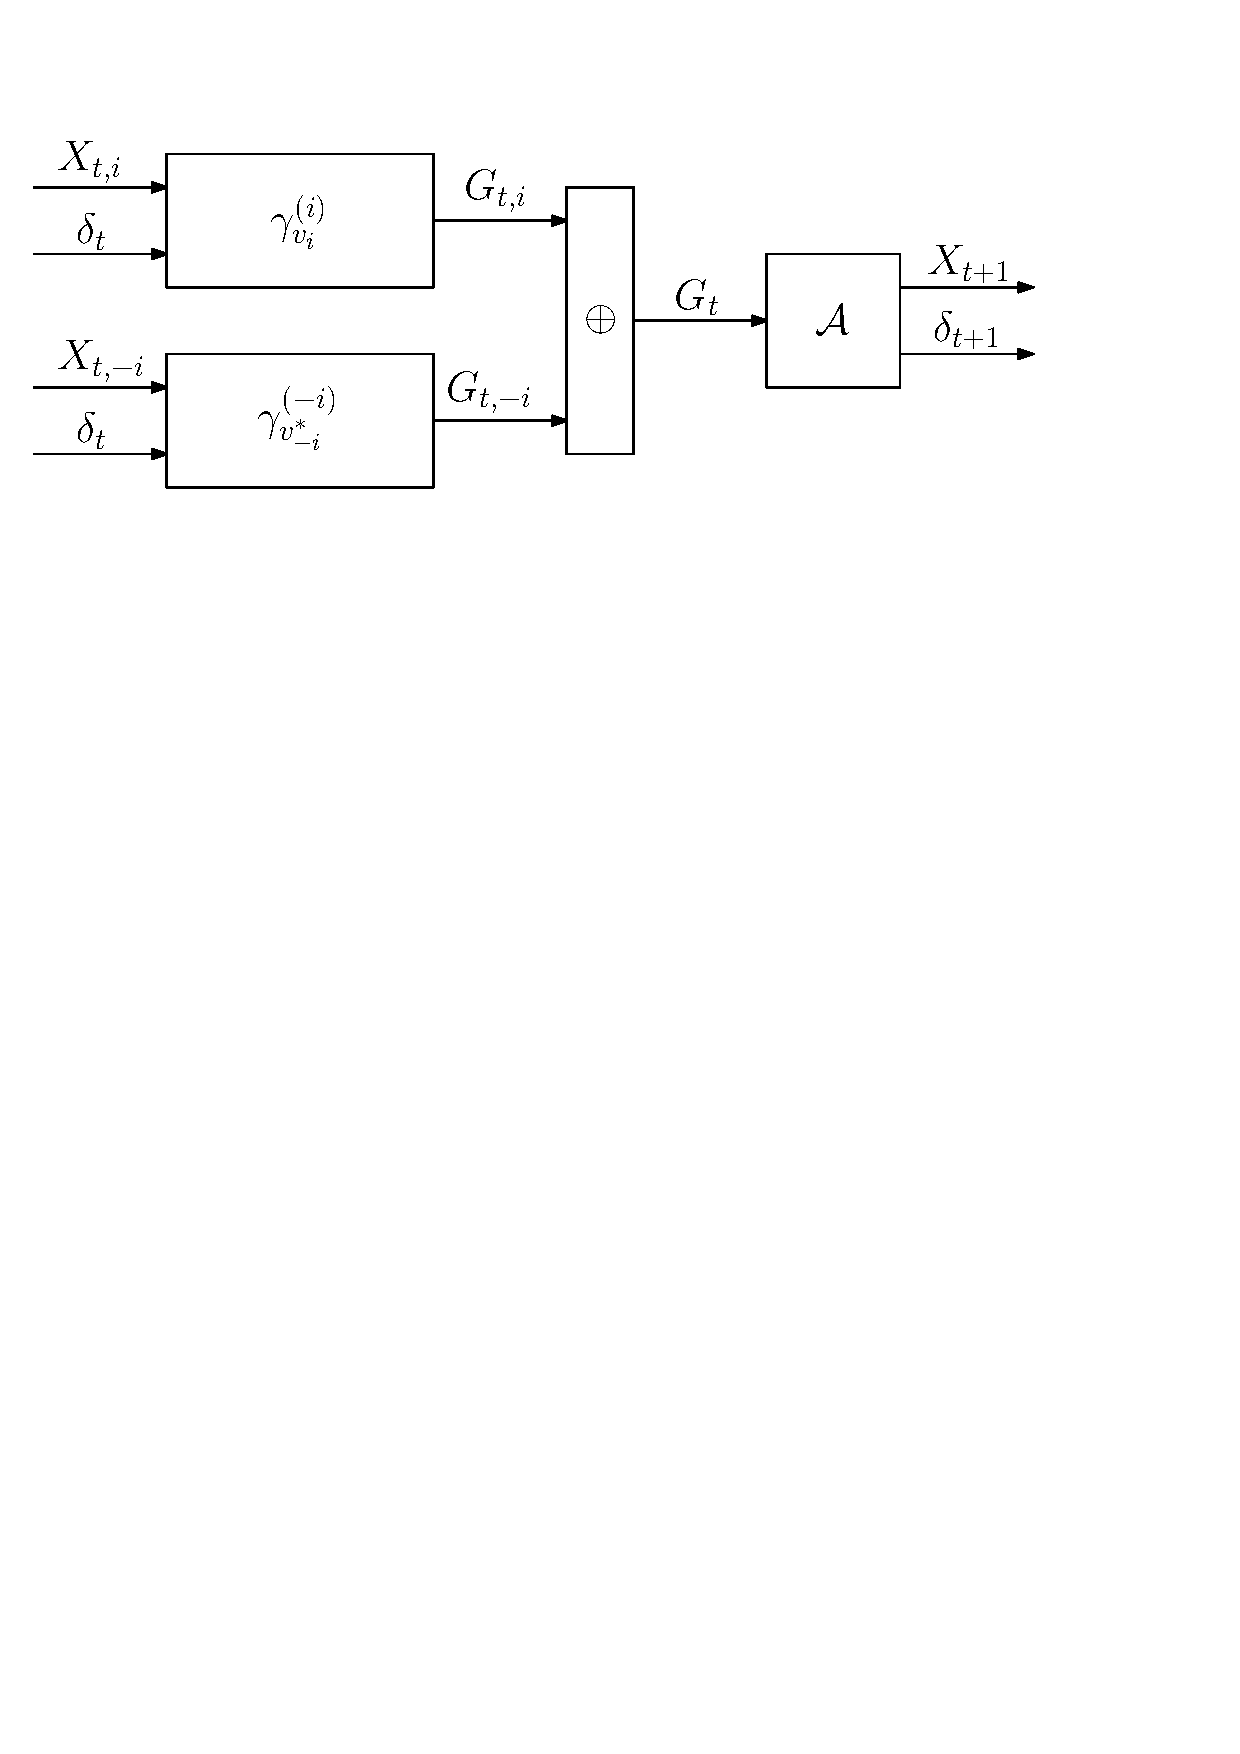
\includegraphics[width=0.5\textwidth]{../figs/ddimto1dim_reduction} % drawn with the IPE app
\end{center}
\caption{The construction of algorithm $\A_i^*$ used in the proof of \cref{lemma:sep}.}
\label{fig:sepalgconstruction}
\end{figure}
\begin{proof}
We will explicitly construct the one-dimensional algorithms, using $\A$. The difficulty is that $\A$ is $d$-dimensional, and the $i$th one-dimensional algorithms can only interact with the one-dimensional oracle
that depends on $v_i$ but does not depend on  $v_{-i}:=(v_1,\ldots,v_{i-1},v_{i+1},\ldots,v_d)$.
Hence, to use $\A$ we need to supply some values $v_{-i}^*$ replacing $v_{-i}$ so that we can use 
the full $d$-dimensional oracle, which $\A$ needs.

Before the construction, we need one more notational convention: 
Slightly abusing notation, we let $v = (v_i,v_{-i})$ and when writing $(v_i,v_{-i})$ as the argument of some function $g$, instead of $g( (v_i,v_{-i}) )$ we will write $g( v_i,v_{-i})$. The decomposition of a vector into one component and all the others will also be used for other $d$-dimensional vectors (not only for $v\in V$).

To define $\A_i^*$, consider the solution of the following max-min problem:
\[
\max_{v_i} \min_{v_{-i}} \tL^{\A}_i(v_i, v_{-i}))\,.
\]
Let the optimal solution of this problem be denoted by $(\hat{v}_i^*,v_{-i}^*)$; we will use $v_{-i}^*$ replacing the missing values $v_{-i}$ when
we create a one-dimensional oracle from a $d$-dimensional.
We also collect $(\hat{v}_i^*)_i$ into the vector $\hat{v}^*\in V^d$.

Now, algorithm $\A_i^*$ is constructed as illustrated on \cref{fig:sepalgconstruction}.
Fix $v_i\in V_i$. Then, algorithm $\A_i^*$ interacts with oracle $\gamma_{v_i}^{(v_i)}$ as follows:
In each round $t$, algorithm $\A_i^*$ produces a pair $(X_t,\delta_t) \in \cK \times [0,1)$. 
In particular, in the first round, $X_1,\delta_1$ is the output of $\A$ in the first round.
In round $t+1$, given the pair $X_t,\delta_t$ produced in the previous round,
the $i$th component of $X_t$ and $\delta_t$ are fed to oracle $\gamma_{v_i}^{(i)}$ (the $i$th component of oracle $\gamma_v$), 
whose output we name $G_{t,i}$. 
The other components of $X_t$, namely $X_{t,-i}$, together with $\delta_t$ are fed to
oracle $\gamma_{v^*_{-i}}^{(-i)}$ which produces a $d-1$-dimensional vector of all but the $i$th component of $\gamma_{(v_i,v^*_{-i})}$, which we call $G_{t,-i}$. 
The values $G_{t,i}$, $G_{t,-i}$ are put together to form the $d$-dimensional vector 
$G_t = (G_{t,i},G_{t,-i})$, which is fed to algorithm $\A$.
We then set $(X_{t+1},\delta_{t+1})$ to be equal to the output of $\A$. 
At the end of the $n$ rounds, $\A$ is queried to produce $\hat{X}_n$, 
whose $i$th component, $\hat{X}_{n,i}$, 
is returned as the output of $\A_i^*$.
\if0
The algorithm will make use of $v_{-1}^*$ (which it does have access to) in the following manner:
Recall that $L$ and $L_1$ are defined as a function of $(\gamma_v)_{v\in \{\pm\}^d}$.
Let $v\in \{\pm 1\}^d$ be fixed, unknown to $\A$ and $\A_1^*$. 
The algorithm construction will make use of $\gamma_v$ and $\gamma_{(1,v_{-1}^*)}$ in the following manner:
At time $t=1$, $\A_1^*$ consults $\A$ to get $\delta$ and the point $X_1\in \cK$.
Next, it asks the oracle $\gamma_v$ for a $d$ dimensional gradient estimate of $f_v$ at $X_1$ with tolerance $\delta$,
obtaining $G_1'$.
At the same time, it also asks $\gamma_{(1,v_{-1}^*)}$ for another $d$ dimensional gradient estimate (this has nothing to do with $f_v$), obtaining $G_1''$.
Then, $G_1 = (G_{1,1}',G_{1,-1}'')$ is fed to $\A$, which returns $X_2\in \cK$. From this point up to the end the process is similar: Both oracles are queried and the gradient to be fed to $\A$ is synthetized by putting together the first component of the gradient estimate from $\gamma_v$ and the last $d-1$ components obtained from $\gamma_{(1,v_{-1}^*)}$.
Finally, at the end, $\A$ produces $\hat{X}_n$, and $\A_1^*$ returns $\hat{X}_{n,1}$.
\fi

By construction, $L^{\A_i^*}_i(v_i) = \tL_i^{\A}(v_i,v_{-i}^*)$.
Now, notice that 
\begin{align*}
\max_{v_i\in V_i} \tL^{\A}_i(v_i,v^*_{-i}) 
=  \tL^{\A}_i(\hat{v}_i^*,v^*_{-i}) 
\le  \tL^{\A}_i(\hat{v}_i^*,\hat{v}^*_{-i})  = \tL^{A}_i(\hat{v}^*)\,,
\end{align*}
where the equality uses the definition of $\hat{v}_i^*$,
while the inequality uses the definition of $v^*_{-i}$.
Thus,
\begin{align*}
\sum_{i=1}^d \max_{v_i\in V_i} L^{\A_i^*}_i(v_i)
%& = \sum_{i=1}^d \max_{v_i\in V_i} \tL^{\A}_i(v_i,v^*_{-i}) 
% = \sum_{i=1}^d  \tL^{\A}_i(\hat{v}_i^*,v^*_{-i}) 
 \le \sum_{i=1}^d  \tL^{\A}_i(\hat{v}^*) 
 = L^{\A}(\hat{v}^*) \le \max_{v\in V } L^{\A}(v)\,,
\end{align*}
which was the claim to be proven.
\end{proof}

Now, let 
\[
\cF^{(i)} = \{f_{v_i} \,:\, v_i\in V\}, \qquad i=1,\dots,d\,.
\] 
%and define
%\[
%\Delta_n^{(d)*} = \Delta^*_{\cF_\sep,n}(c_1, c_2 )\,.
%\]
The next result follows easily from the previous lemma:
\begin{lemma}
\label{lem:sep2}
Let $\norm{\cdot} =\norm{\cdot}_2$ in the definition of the type-I oracles.
%Let $\inf_{x\in \cK_i} f_{v_i}^{(i)}(x) = 0$. 
Then, we have that 
\[
\Delta^*_{\cF_\sep,n}(c_1, c_2 ) \ge \sum_{i=1}^d \Delta_{\cF^{(i)},n}^*(c_1/\sqrt{d},c_2/d)\,.
\]
\end{lemma}
\begin{proof}
By our earlier remark, $\Gamma_\sep(f_v,c_1/\sqrt{d},c_2/d) \subset \Gamma(f,c_1,c_2)$. Hence,
\begin{align*}
\Delta^*_{\cF_\sep,n}(c_1, c_2 ) 
	& = \inf_{\cA} \sup_{v\in V} \sup_{\gamma \in \Gamma(f_v,c_1,c_2)} \Delta^{\cA}_n(f_v,\gamma) 
	 \ge \inf_{\cA} \sup_{v\in V} \sup_{\gamma \in \Gamma_\sep(f_v,c_1/\sqrt{d},c_2/d)} \Delta^{\cA}_n(f_v,\gamma)\,.
	 \numberthis
	 \label{eq:ddimtoonedim1}
\end{align*}
For each $i=1,\dots,d$, pick $\gamma_{v_i}^{(i)}\in \Gamma(f_{v_i},c_1/\sqrt{d},c_2/d)$ such that 
$\Delta_n^*(\cF^{(i)},c_1/\sqrt{d},c_2/d) = \inf_{\cA} \sup_{v_i\in V_i} \Delta_n^{\cA}(f_{v_i},\gamma_{v_i}^{(i)})$.
For $v \in V$, let $\gamma_v \in \Gamma_\sep(f_v,c_1/\sqrt{d},c_2/d)$ be the oracle whose ``components'' are 
$\gamma_{v_i}^{(i)}$, $i=1,\dots,d$.
Now, by \cref{lemma:sep},
\begin{align*}
\sup_{v\in V} \Delta^{\cA}_n(f_v,\gamma_v)
\ge
\sum_{i=1}^d \inf_{\cA} \sup_{v_i\in V_i} \Delta^{\cA}_n(f_{v_i}^{(i)},\gamma_{v_i}^{(i)})
=
\sum_{i=1}^d  \Delta_{\cF^{(i)},n}^*(c_1/\sqrt{d},c_2/d)\,.
\end{align*}
This, together with 
$\sup_{v\in V} \sup_{\gamma \in \Gamma_\sep(f_v,c_1/\sqrt{d},c_2/d)} \Delta^{\cA}_n(f_v,\gamma)
\ge \sup_{v\in V} \Delta^{\cA}_n(f_v,\gamma_v)$
and \eqref{eq:ddimtoonedim1} gives the desired result.
\end{proof}

\paragraph{Main proof:}
Let $\cK \subset \R^d$, such that $\times_i \cK_i \subset \cK$, $\{\pm 1 \} \subset \cK_i \subset \R$,
$\F_d = \F_{L,0}(\K)$, where recall that $L\ge 1/2$.
 For any $1\le i \le d$, $x_i \in \cK_i$, 
\begin{align}
\label{eq:smoothddim}
%  f_v(x) :=& \sum_{i=1}^d f^{(i)}_{v_i}(x_i), \,\,  \text{ where }
  f^{(i)}_{v_i}(x_i) := \epsilon\left( x_i-v_i\right)+2\epsilon^2 \ln\left(1+e^{-\frac{x_i-v_i}{\epsilon}}  \right)\,.
\end{align}
i.e., $f^{(i)}_{v_i}$ is like in the one-dimensional lower bound proof (cf. equation~\ref{eq:fvdef}).
Note that $f_v \in \F_d$ since $f_v$ is separable, so its Hessian is diagonal and from our earlier calculation
we know that
$0\le \frac{\partial^2}{\partial x_i^2} f^{(i)}_{v_i}(x_i) \le 1/2$.
Let $\Delta_n^{(d)*}$ denote the minimax error $\Delta_{\F_d, n}^*\left(C_1\delta^p,\frac{C_2}{\delta^q}\right)$ for the $d$-dimensional family of functions $\F_d$. 
Let $\F^{(i)} = \{ f^{(i)}_{-1},  f^{(i)}_{+1} \}$.
As it was noted above, $f_v\in \F_d$ for any $v\in \{\pm 1\}^d$.
Hence, by~\cref{lem:sep2}, 
\begin{align*}
 \Delta_n^{(d)*} &\ge \sum_{i=1}^d \Delta_{\F^{(i)},n}^{*}\left(\frac{C_1}{\sqrt{d}}\, \delta^p, \frac{C_2}{d} \delta^{-q}\right)\,.
               \numberthis \label{eq:dlb}
\end{align*}

% Fix an $i$ and consider the loss $L_i(v)$.
% We now argue that, since $f_v$ is separable, any algorithm $\A$ that uses information in dimensions other than $i$ in the gradient samples of the oracle, can be replaced by $d$ algorithms $\A_1^*$, $\dots$, $\A_d^*$ such that $\A_i^*$ is only using information for dimension $i$ and is only predicting the $i$th coordinate at the end, and the sum of losses they incur is utmost that of $\A$ in the worst-case.
\if0
The minimax error $\Delta_n^{(d)*}$ can be lower bounded as follows:
\begin{align}
\Delta_n^{(d)*}  &\ge  \inf_{\A} \max_{v\in {\pm 1}^d} L^\A(v) \nonumber\\
 & \ge \inf_{\A_1} \max_{v_1\in \{\pm 1\}} L_1^{\A_1}(v_1) + \dots + 
 			\inf_{A_d} \max_{v_d\in \{\pm 1 \}} L_d^{\A_d}(v_d) \label{eq:splitA}\\
%             \ge & \inf_{\A_1^*} L_1(v^*) + \ldots + \inf_{\A_d^*} L_d(v^*) \label{eq:splitA}\\
               & \ge d \Delta_n^{*}\left(\F_1,\frac{C_1\delta^p}{\sqrt d}, \frac{C_2}{d\delta^q}\right)\,, \label{eq:dlb}
\end{align}
where in inequality \eqref{eq:splitA}, algorithms $\A_i$ are interacting with the respective one-dimensional oracles $\gamma^{(i)}_{v_i}$ only 
and the inequality follows by~\eqref{eq:onedimlb},
while the inequality \eqref{eq:dlb} follows from the fact that each infimum term in \eqref{eq:splitA} is solving a $1$-dimensional problem and hence the bound in \eqref{eq:final-lower-bd} applies with $C_1$ replaced by $C_1/\sqrt{d}$ and $C_2$ replaced by $C_2/d$. The resulting bound is denoted by $\Delta_n^{*}\left(\F_1,\frac{C_1\delta^p}{\sqrt d}, \frac{C_2}{d\delta^q}\right)$. 
\fi
% is the one-dimensional minimax error, which is lower-bounded in \eqref{eq:final-lower-bd}. \todoc{However, I would have written just the $1$d final bound there, or $\Delta_n^*( \dots )$ with some notation, because we don't want to redo this whole optimization business..}

% Using the one-dimensional minimax error $\Delta_n^{*}$, we obtain
% \[\Delta_n^* \ge d \Delta_n^{*}.\]
\paragraph{Derivation of rates:}\ \\
Plugging the lower bound derived in \eqref{eq:lb-pq} for the one-dimensional setting into the bound in \eqref{eq:dlb}, we obtain a $\sqrt{d}$-times bigger lower bound for the $d$-dimensional case for any $p, q >0$:
\begin{align}
\Delta_n^{(d)*} \ge  \sqrt{d} \frac{\left(2p+q\right)^2}{2q^{\frac{q}{2p+q}}\left(4p+q\right)^{\frac{4p+q}{2p+q}}}C_1^{\frac{q}{2p+q}} C_2^{\frac{p}{2p+q}}  n^{-\tfrac{p}{2p+q}} \,.
\label{eq:lb-pq-1}
\end{align}
The above bound simplifies to the following for the case where $p=1$ and $q=2$:
\begin{align*}
% \Delta_n^{*}\left(\F_1,\frac{C_1\delta^p}{\sqrt d}, \frac{C_2}{d\delta^q}\right) \ge &\frac{1}{2}\sqrt{\frac{C_1 C_2}{2 d^{\frac{3}{2}}}} n^{-1/4} \text{ and hence,} \\
\Delta_n^{(d)*}  \ge& \dfrac{ 2(C_1^2C_2)^{1/4}}{3\sqrt{3}} \sqrt{d}n^{-1/4}.
\end{align*}

On the other hand, for the case $p=q=2$, we obtain
\begin{align*}
% \Delta_n^{*}\left(\F_1,\frac{C_1\delta^p}{\sqrt d}, \frac{C_2}{d\delta^q}\right) \ge &\dfrac{3}{8}\left(\frac{C_1 C_2^2}{16 d^{\frac{5}{2}}}\right)^{1/3} n^{-1/3} \text{ and hence,} \\
\Delta_n^{(d)*}  \ge& \frac{9}{10}\left(\frac{C_1 C_2}{25}\right)^{1/3} \sqrt{d}n^{-1/3}.
\end{align*}

\subsection{Proof of Theorem \ref{thm:lb-convex} for strongly convex + smooth function class $\F_{L,1}(\K)$.}
\label{sec:appendix-lbscconvex}
We follow the notational convention used earlier for convex functions in one dimension. 
Let $\F = \F_{L,1}(\K)$, where $L\ge 1$ and $\K$  contains $\pm 1$.
We consider functions $f_v$, for $v \in \{-1,+1\}$, defined as
\begin{align}
  f_v(x) := \dfrac{1}{2} x^2 - v\epsilon x \,,\quad x \in \cK\,.
  \label{eq:socfdef}
\end{align}
It is easy to see that $\{f_+, f_-\}\subset \F$.
%%%%%%%%%%%%%%%%%%%%%%%%%%%%%%%%%%%%%%%%%%%%%%%%%%%%%%%%%%%%%%%%%%%%%%%%%%%%%%% 

Clearly, $f_v$ is minimized at $x^*_v = v\epsilon$.
By the definition of $f_v$, we have
%Using the fact that $f_+$ and $f_-$ are strongly convex with associated constant $\left(\dfrac{\epsilon}{2}\right)$, we obtain
\begin{align}
  f_v(x) - f_v(x^*_v)
\ge  \dfrac{\epsilon^2}{2}  \indic{x v  < 0}. \label{eq:fv-lb-sc}
\end{align}
We will consider the oracles $\gamma_v$ defined as 
\begin{align}
 \gamma_v(x) = x-v\epsilon + v \min(\epsilon,C_1 \delta^p) + \xi, \label{eq:oracle-1d}
\end{align}
where $\xi \sim \normal(0,\frac{C_2}{\delta^q})$; as with $f_v$, we will also use $\gamma_{+}$ ($\gamma_-$) 
to denote $\gamma_{+1}$ (resp., $\gamma_{-1}$).
The oracle is indeed a $(c_1,c_2)$ type-I oracle, with $c_1(\delta)=C_1\delta^p$ and $c_2(\delta)=\frac{C_2}{\delta^q}$.
%%%%%%%%%%%%%%%%%%%%%%%%%%%%%%%%%%%%%%%%%%%%%%%%%%%%%%%%%%%%%%%%%%%%%%%%%%%%%%% 

Using arguments similar to those in the proof of lower bound for convex functions, we obtain
\begin{align}
\Delta_n^{(1)*}:=\Delta_n^{*} %\nonumber\\
  \ge  &\inf_{\A} \dfrac{\epsilon^2 }{2}  \,\left( 1 - \left(\frac12\dkl{P_{+}}{P_{-}}\right)^{\frac{1}{2}}\right), \label{eq:pinskersc}
\end{align}
Note that $P_+$ (resp. $P_-$) is $\P$ conditioned on the event $V=+1$ (resp. $V=-1$).
%, since $v$ takes values in $\{+\nu,-\nu\}$. The conditioning in the earlier proof for convex function was on $V=+1$ for $P_+$ as $v$ there was taking values $\{+1,-1\}$.
%%%%%%%%%%%%%%%%%%%%%%%%%%%%%%%%%%%%%%%%%%%%%%%%%%%%%%%%%%%%%%%%%%%%%%%%%%%%%%% 

Observe that, for any $x\in \R$, $f_-'(x) - f_+'(x) = 2\epsilon$ and hence
\begin{align}
 |\gamma_+(x) - \gamma_-(x)| 
& = | f'_+(x) - \min(\epsilon,C_1 \delta^p) - (f'_-(x)+\min(\epsilon,C_1 \delta^p)) | 
 = 2 (\epsilon - C_1 \delta^p)^+.
 \label{eq:gdiff-ub-sc}
\end{align}
From the foregoing, 
\begin{align}
 \MoveEqLeft \dkl{P_{+}^t(\cdot\mid g_{1:t-1})}{P_{-}^t(\cdot\mid g_{1:t-1})}
 \le  \dfrac{2\{(\epsilon-C_1\delta_t^p)^+\}^2\delta_t^q}{{C_2}},\label{eq:dkgausssc}
\end{align}
where the inequality \eqref{eq:dkgausssc} follows from \eqref{eq:gdiff-ub-sc}.
Thus, we obtain
\begin{align}
\dkl{P_{+}}{P_{-}} \le 2n \sup_{\delta>0} \dfrac{\{(\epsilon-C_1\delta^p)^+\}^2 \delta^q}{C_2}.
\label{eq:kluboundsc}
\end{align}
Substituting the above bound into \eqref{eq:pinskersc}, we obtain 
\begin{align}
 \Delta_n^{(1)*}
  \ge & \dfrac{\epsilon^2}{2} \left(1 - \sqrt{
    n}  \sup_{\delta>0}\dfrac{(\epsilon-C_1\delta^p)^+\delta^{q/2}}{\sqrt{C_2}}
  \right)\,.\label{eq:final-lower-bd-sc}
\end{align}


\paragraph{Derivation of the rates uniformly for all $\delta$:}
As in the proof of the lower bound for $\F_{L,0}(\K)$, we replace the positive part function in \eqref{eq:final-lower-bd-sc} and optimize over $\delta$ to obtain
that the right-hand side of~\eqref{eq:kluboundsc} is optimized by
\begin{align}
\delta_*=\left(\frac{ \epsilon q}{C_1(2p+q)}\right)^{1/p}\,.
\label{eq:deltastar-sc}
\end{align}
%where $z=p/q$. Recall that we require $\nu/C_1 \ge {\delta^*}^p$, which results in the condition on $\nu$ above.

From the above, we have 
% and for any choice of $\delta$, the minimax error $\Delta_n^{*}$ satisfies
\[
\Delta_n^{(1)*} \ge \dfrac{\epsilon^2}{2} \left(1 - \sqrt{
    n}  \dfrac{ (\epsilon-C_1\delta_*^p)\delta_*^{q/2}}{\sqrt{C_2}}
  \right)= \dfrac{\epsilon^2}{2} \left(1 - \sqrt{n}  K_1 \epsilon^{\frac{p+\tfrac{q}{2}}{p}}\right)\,, 
\]
 where $K_1 = \dfrac{p}{\sqrt{C_2}(p+\tfrac{q}{2})} \left(\dfrac{q}{2C_1(p+\tfrac{q}{2})}\right)^{\frac{q}{2p}}$.

Plugging in $\epsilon = \left(\dfrac{4p}{(6p+q)\sqrt{n} K_1} \right)^{\frac{2p}{2p+q}}$, we obtain
\begin{align}
\Delta_n^{(1)*} \ge 2^{\frac{2p-q}{2p+q}} \frac{(2p+q)^3}{q^{\frac{2q}{2p+q}}(6p+q)^{\frac{6p+q}{2p+q}}}  C_1^{\frac{2q}{2p+q}}C_2^{\frac{2p}{2p+q}} n^{-\frac{2p}{2p+q}}.
\label{eq:lb-pq-sc}
\end{align}
%The above bound holds for $n$ such that 
%$$\!d^{\frac{-(4p+q)}{(2p+q)}}\!\!\left(\frac{1}{2\sqrt{n} K_1} \right)^{\!\!\frac{p}{p+\frac{q}{2}}} \!\!\!\le \!\!\min\!\left( \frac{C_1 (2p+q)}{q}, \frac{2z+1}{C_1^{2z-1}(z+1)^z}\!\right).$$
%As in the proof of the lower bound for $\F_{L,0}(\K)$, the first condition on $n$ above is due to the assumption that $\delta \le 1$ in Definition \ref{def:oracle1}, while the second condition is due to the constraint on $\nu$ in \eqref{eq:deltastar-sc}.

Now, when $q=2$ and $p=1$, the lower bound in \eqref{eq:lb-pq-sc} simplifies to
\[
\Delta_n^{(1)*} \ge \frac{1}{2} C_1 C_2^{1/2} n^{-1/2}.
\]
On the other hand, for $p=q=2$, we obtain
\[
\Delta_n^{(1)*} \ge 27\left(\frac{2}{7^7}\right)^{\frac{1}{3}} C_1^{2/3}C_2^{2/3} n^{-2/3} .
\]


%%%%%%%%%%%%%%%%%%%%%%%%%%%%%%%%%%%%%%%%%%%%%%%%%%%%%%%%%%%%%%%%%%%%%%%%%%%%%%%
%%%%%%%%%%%%%%%%%%%%%%%%%%%%%%%%%%%%%%%%%%%%%%%%%%%%%%%%%%%%%%%%%%%%%%%%%%%%%%%

\paragraph{Generalization to $d$ dimensions:}
Recall that in this result, $\norm{\cdot} = \norm{\cdot}_2$.
The proof in $d$ dimensions for strongly convex functions is the same as that for the case of smooth convex functions
with the difference that we use~\eqref{eq:socfdef} in defining the functions $f^{(i)}_{v_i}$.
Then, for any $v\in \{\pm 1 \}^d$, $f_v\in \F_{L,1}(\cK)$. Indeed, $f_v(x) = \sum_{i=1}^d f^{(i)}(x_i)$,
hence $\nabla^2 f_v(x) =  I_{d\times d}$, where $I_{d\times d}$ is the $d\times d$ identity matrix.
Thus, $\lambda_{\min}(\nabla^2 f_v(x)) = \lambda_{\max}(\nabla^2 f_v(x)) = 1$.
From~\eqref{eq:dlb} and~\eqref{eq:lb-pq-sc} we get
\begin{align}
\Delta_n^{(d)*} \ge \Delta_n^{(1)*} \,.
%\dfrac{1}{4} d^{\frac{-2p}{(2p+q)}} \left(\dfrac{1}{2 K_1 \sqrt n}\right)^{\frac{2p}{p+\frac{q}{2}}} \text{ for } 
%\nu = d^{\frac{-(4p+q)}{(2p+q)}}\left(\dfrac{1}{2\sqrt{n} K_1} \right)^{\frac{p}{p+\frac{q}{2}}}.
\label{eq:lb-pq-d}
\end{align}

%Case $p=1$ and $q=2$:
%\begin{align*}
%% \Delta_n^{*}\left(\F_1,\frac{C_1\delta^p}{\sqrt d}, \frac{C_2}{d\delta^q}\right) \ge &\frac{1}{2}\sqrt{\frac{C_1 C_2}{2 d^{\frac{3}{2}}}} n^{-1/4} \text{ and hence,} \\
%\Delta_n^{(d)*}  \ge& \dfrac{C_1 C_2}{2} n^{-1/2} d^{-1/2}.
%\end{align*}
%
%Case $p=q=2$:
%\begin{align*}
%% \Delta_n^{*}\left(\F_1,\frac{C_1\delta^p}{\sqrt d}, \frac{C_2}{d\delta^q}\right) \ge &\dfrac{3}{8}\left(\frac{C_1 C_2^2}{16 d^{\frac{5}{2}}}\right)^{1/3} n^{-1/3} \text{ and hence,} \\
%\Delta_n^{(d)*}  \ge& \frac{9}{4}\left(\frac{C_1^2 C_2^4}{16}\right)^{1/3} n^{-2/3} d^{-2/3}.
%\end{align*}



%%% Local Variables: 
%%% mode: latex
%%% TeX-master: "bgo"
%%% End: 
